
%%%%%%%%%%%%%%%%%%%%%%%InSTA2015の論文
\chapter{I/O テストデータパターンを使ったテストケース抽出手法}\label{chap:4}
本章では,テスト分析において,テスト条件を網羅的に特定し,テストケースを抽出する方法として,テスト実行時のデータの入出力(以降I/Oと呼ぶ)に着目する.
テストベースを分析する際に,テスト実行時のI/Oの要素で分解し網羅性を確認する方法を提案する.
\newpage

\section{研究の概要} \label{sec:4-1}
\subsection{研究の目的} \label{sec:4-1-1}


しかしながら,テストベースの分析に論理的機能構造をガイドとして使用することを明示しているだけであり,具体的な分析手順について定義できていない.そのため,実験の際に被験者に対して,テスト分析にて仕様項目の選択を網羅的に行う具体的な方法を明確に提示できていない.

\subsection{I/Oテストデータパターン} \label{sec:4-1-1}
テストを実行するためには,データをテスト対象にインプットし,テスト対象のアウトプットを期待結果と実際の結果で比較する.

たとえば,シンプルな機能の四則演算の計算結果が正しいことを検証するときには,テスト対象の外部から複数の値を入力し,テスト対象がそれらの値を計算し,計算結果をテスト対象の外部にアウトプットする.

これは図~\ref{fig:D-3-Fig4}で示している「外部からのデータ入力,外部へのデータ出力」というパターンになる.

また,固定比率が計算結果に適用されるとき(他の計算も適用されると言う意味で),テスト対象は適切な比率を呼び出し,利用してから計算結果をアウトプットする.
これは図〜\ref{fig:D-4-Fig5}で示している例「外部と内部からのデータ入力,外部へのデータ出力」となる.
\begin{figure}[htbp]
 \begin{center}
 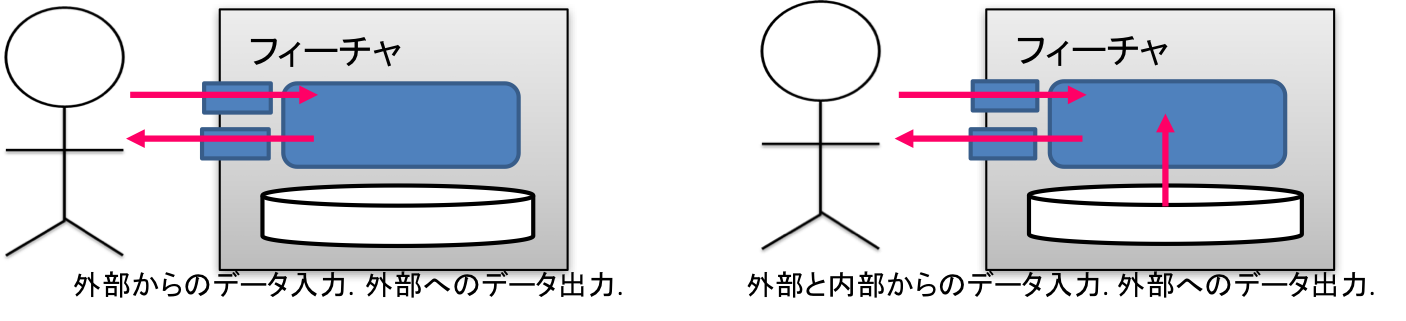
\includegraphics[width=10cm]{./image/D-3-Fig4.png}
 \caption{テスト対象へのデータ入出力の説明}
 \label{fig:D-3-Fig4}
 \end{center}
\end{figure}
注意すべきこととしてI/Oデータパターンはテスト対象の外部からの観察が可能なものを選ぶことがあげられる.
処理の起動終了に使われる内部のコマンド(シグナルやイベント)は,データパターンへ分類をするときに考慮しない.
なぜならこの手法はブラックボックステストのためのテストベースの分析手法であり,AUT内部のシグナルやイベントのような内部コマンドは,システムテストレベルでのブラックボックステストでは,明示的に考慮しないからである.


テスト実行をするときのテスト対象へのデータのインプットの方法は,外部からの入力,内部に保持したデータの入力,外部と内部からの入力の3パターンに分類できる.
同じようにテスト対象からのアウトプット方法は外部への出力,内部に保持したデータの出力,外部と内部からデータの出力の3パターンに集約でき,入出力の組み合わせ数はすべてで9パターンとなる.
\begin{figure}[htbp]
\begin{center}
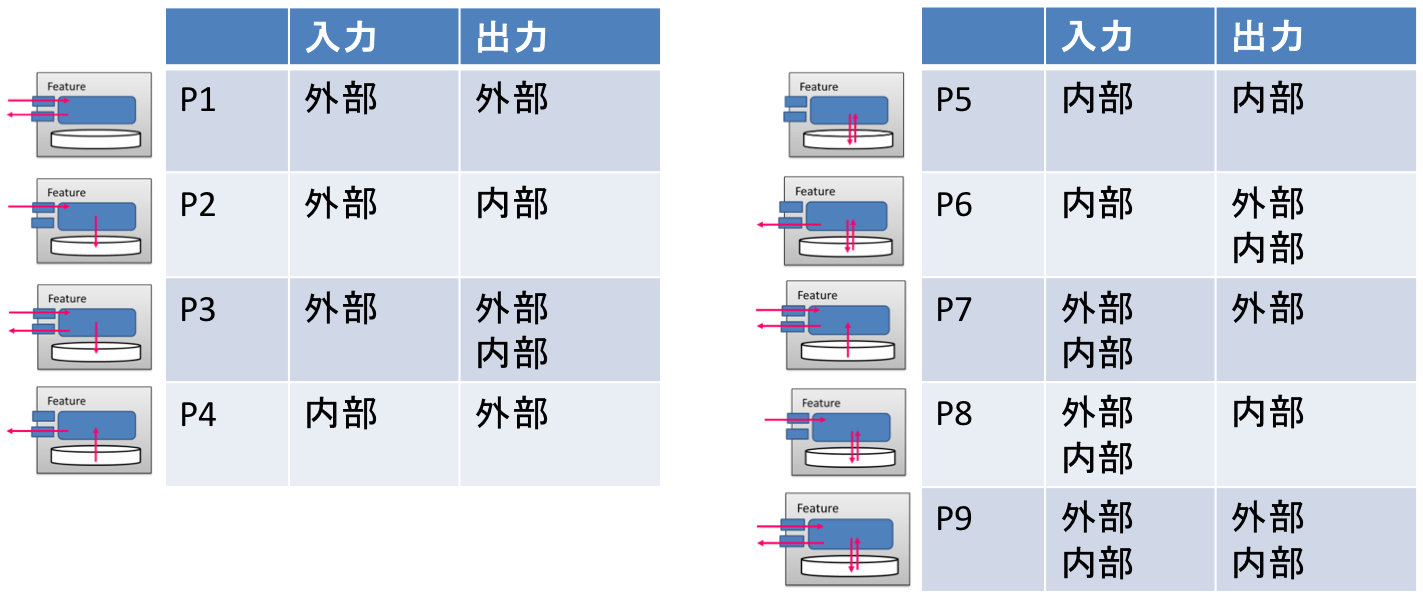
\includegraphics[width=14cm]{./image/D-3-Fig5.png}
\caption{I/Oデータパターン}
\label{fig:D-4-Fig6}
\end{center}
\end{figure}

テスト対象に対するテスト実行時のデータの入出力をまとめたパターンは図~\ref{fig:D-4-Fig6}のように9パターンに集約できる.
これをI/Oテストデータパターンと呼ぶ.
I/Oテストデータパターンがテスト実行時のデータの入出力から見た全体集合となる.

Whittakerによって提案されているフォールトモデル\cite{whittaker2003break}は,AUTの入力と出力のモデルに関する類似の研究である.フォールトモデルの目的はフォールトを見つけることであり,AUTの入出力モデルはテストベースから特定するテスト条件である,仕様項目を分類するモデルとして使われる.

テスト分析のアウトプットである仕様項目は最終的に全て実行して確認することができなければならないので,全てが9パターンのどれかに分類できる.

\subsection{I/Oテストデータパターンとテストカテゴリ}

検証実験からの結果をI/Oデータパターンに分類するために,P1からP9の識別子を仕様項目の属性として付与した.その後,3章の表~\ref{tbl:D-3-tbl4}で示した評価レベルのアプローチをベースに整理した.

実験結果は表~\ref{tbl:D-3-tbl7}と表~\ref{tbl:D-3-tbl8}に示したとおりである.前節の結果と本節の結果では行数が異なるの理由は, 仕様項目のいくつかは同じテストカテゴリに属する仕様項目でも異なったI/Oデータパターンを付与している場合があり,そのためテストカテゴリを論理構造の項目で集約をしていないためである.表~\ref{tbl:D-3-tbl7}と表~\ref{tbl:D-3-tbl8}が示すとおり, P1, P2, P4, P7 が検証実験で使ったAUTに対応するデータパターンであった.

% Table generated by Excel2LaTeX from sheet 'データの入出力ごとフェリカ (掲載用加工)'
\begin{table}[htbp]
\centering
\caption{Fig. 8-1. The evaluation results of the I/O data pattern.}
  \begin{tabular}{|l|l|l|r|l|l|l|l|l|l|}
  \hline
  \multicolumn{2}{|c}{\multirow{2}[4]{*}{Logical
Structure}} & \multicolumn{1}{r}{} &       & \multicolumn{6}{c|}{Team} \bigstrut\\
\cline{5-10}    \multicolumn{2}{|c}{} & \multicolumn{1}{r}{} &       & TM1   & TM2   & TM3   & TM4   & TM5   & TM6 \bigstrut\\
  \hline
  \textbf{Conv} & P1    & ボリューム強弱 &       & -     & -     & -     & -     & -     & - \bigstrut\\
  \hline
  \textbf{Conv} & P1    & 対向機   &       & B     & A+    & B     & B     & B     & - \bigstrut\\
  \hline
  \textbf{Support} & P1    & 状態遷移  &       & B     & B     & B     & B     & B     & B \bigstrut\\
  \hline
  \textbf{Mngt} & P1    & 電話と音楽の音量の影響 &       & B     & A+    & A+    & A+    & A+    & A+ \bigstrut\\
  \hline
  \textbf{Storage} & P2    & ボリューム値保存 &       & -     & A+    & -     & A+    & A+    & - \bigstrut\\
  \hline
  \textbf{Conv} & P4    & デフォルト値/設定値 &       & B     & B     & B     & B     & -     & B \bigstrut\\
  \hline
  \textbf{Mngt} & P4    & リセット  &       & B     & B     & B     & A+    & B     & A+ \bigstrut\\
  \hline
  \textbf{Output} & P7    & ビープ音  &       & -     & -     & -     & -     & -     & A+ \bigstrut\\
  \hline
  \end{tabular}%
\label{tbl:D-3-tbl7}%
\end{table}%

% Table generated by Excel2LaTeX from sheet 'データの入出力ごとフェリカ (掲載用加工)'
\begin{table}[htbp]
\centering
\caption{Fig. 8-2. The evaluation results of the I/O data pattern.}
  \begin{tabular}{|l|l|l|l|l|}
  \hline
  \multicolumn{3}{|c|}{\multirow{2}[4]{*}{Logical
Structure}} & \multicolumn{2}{c|}{Team} \bigstrut\\
\cline{4-5}    \multicolumn{3}{|c|}{} & TM1   & TM2 \bigstrut\\
  \hline
  \textbf{Input} & P1    & P1    & B     & B \bigstrut\\
  \hline
  \textbf{Support} & P1    & P1    & -     & A+ \bigstrut\\
  \hline
  \textbf{Support} & P1    & P1    & B     & B \bigstrut\\
  \hline
  \textbf{Storage} & P2    & P2    & A+    & A+ \bigstrut\\
  \hline
  \textbf{Input} & P4    & P4    & -     & - \bigstrut\\
  \hline
  \textbf{Mngt} & P4    & P4    & B     & A \bigstrut\\
  \hline
  \textbf{Output} & P4    & P4    & B     & B \bigstrut\\
  \hline
  \textbf{Output} & P4    & P4    & A     & A \bigstrut\\
  \hline
  \textbf{Input} & P7    & P7    & A     & - \bigstrut\\
  \hline
  \textbf{Conv} & P7    & P7    & A     & A \bigstrut\\
  \hline
  \textbf{Output} & P7    & P7    & B     & B \bigstrut\\
  \hline
  \end{tabular}%
\label{tbl:D-3-tbl8}%
\end{table}%

%The summarized results of the I/O data pattern are shown in Fig.9.  The percentage of combined scores of A and A+ for each input-output pattern have been recorded. P2 is 100percent for both the experiments. It can be said that P2 has had the most significant result.
I/Oデータパターンで集約した結果を表~\ref{tbl:D-3-tbl9}と表~\ref{tbl:D-3-tbl10}である.各I/Oデータパターンにて A and A+ の割合を確認すると,P2のみが両方の検証実験で100%となったため,P2のデータパターンに対する効果が最も高い.

音楽再生機器の場合,P2に分類された仕様項目はボリューム値の保存である.この仕様項目はテストベースに記述はされているものの,ボリュームコントロールのセクションとは別のセクションに記述されていた.飛行機予約システムの場合,P2に分類された仕様項目は注文内容のデータベースへの保存である. データベースへの保存に関して,テストベースには,詳しい記載は無かった. これらの観察結果はセクションIIIに前述した推測である「明白に必要だと思われる仕様の一部分が記述されていない.」と一致している.


% Table generated by Excel2LaTeX from sheet 'データの入出力ごとフェリカ (掲載用加工)'
%Fig. 9-1. The summarized results of the I/O data patterns.
\begin{table}[htbp]
\centering
\caption{The summarized results of the I/O data patterns.}
  \begin{tabular}{lrrrrrr}
\cline{1-6}    \multicolumn{1}{|c}{\multirow{2}[4]{*}{I/O pattern }} & \multicolumn{1}{r|}{} & \multicolumn{4}{c|}{Evaluation level} &  \bigstrut\\
\cline{3-6}    \multicolumn{1}{|c}{} & \multicolumn{1}{r|}{} & \multicolumn{1}{l|}{A+} & \multicolumn{1}{l|}{A} & \multicolumn{1}{l|}{-} & \multicolumn{1}{l|}{B} &  \bigstrut\\
\cline{1-6}    \multicolumn{1}{|l|}{P1} & \multicolumn{1}{r|}{} & \multicolumn{1}{r|}{6} & \multicolumn{1}{r|}{0} & \multicolumn{1}{r|}{7} & \multicolumn{1}{r|}{11} & 35.3\% \bigstrut\\
\cline{1-6}    \multicolumn{1}{|l|}{P2} & \multicolumn{1}{r|}{} & \multicolumn{1}{r|}{3} & \multicolumn{1}{r|}{0} & \multicolumn{1}{r|}{3} & \multicolumn{1}{r|}{0} & 100.0\% \bigstrut\\
\cline{1-6}    \multicolumn{1}{|l|}{P4} & \multicolumn{1}{r|}{} & \multicolumn{1}{r|}{2} & \multicolumn{1}{r|}{0} & \multicolumn{1}{r|}{1} & \multicolumn{1}{r|}{9} & 18.2\% \bigstrut\\
\cline{1-6}    \multicolumn{1}{|l|}{P7} & \multicolumn{1}{r|}{} & \multicolumn{1}{r|}{1} & \multicolumn{1}{r|}{0} & \multicolumn{1}{r|}{5} & \multicolumn{1}{r|}{0} & 100.0\% \bigstrut\\
\cline{1-6}    the persentage = (A+  +  A) /(A+  +  A + B)  &       &       &       &       &       &  \bigstrut[t]\\
  \end{tabular}%
\label{tbl:D-3-tbl9}%
\end{table}%

% Table generated by Excel2LaTeX from sheet 'データの入出力ごとフェリカ (掲載用加工)'
\begin{table}[htbp]
\centering
\caption{The summarized results of the I/O data patterns}
  \begin{tabular}{lrrrrrr}
\cline{1-6}    \multicolumn{1}{|c}{\multirow{2}[4]{*}{I/O pattern}} & \multicolumn{1}{r|}{} & \multicolumn{4}{c|}{Evaluation level} &  \bigstrut\\
\cline{3-6}    \multicolumn{1}{|c}{} & \multicolumn{1}{r|}{} & \multicolumn{1}{l|}{A+} & \multicolumn{1}{l|}{A} & \multicolumn{1}{l|}{-} & \multicolumn{1}{l|}{B} &  \bigstrut\\
\cline{1-6}    \multicolumn{1}{|l|}{P1} & \multicolumn{1}{r|}{} & \multicolumn{1}{r|}{1} & \multicolumn{1}{r|}{0} & \multicolumn{1}{r|}{1} & \multicolumn{1}{r|}{4} & 20.0\% \bigstrut\\
\cline{1-6}    \multicolumn{1}{|l|}{P2} & \multicolumn{1}{r|}{} & \multicolumn{1}{r|}{2} & \multicolumn{1}{r|}{0} & \multicolumn{1}{r|}{0} & \multicolumn{1}{r|}{0} & 100.0\% \bigstrut\\
\cline{1-6}    \multicolumn{1}{|l|}{P4} & \multicolumn{1}{r|}{} & \multicolumn{1}{r|}{0} & \multicolumn{1}{r|}{3} & \multicolumn{1}{r|}{2} & \multicolumn{1}{r|}{3} & 50.0\% \bigstrut\\
\cline{1-6}    \multicolumn{1}{|l|}{P7} & \multicolumn{1}{r|}{} & \multicolumn{1}{r|}{0} & \multicolumn{1}{r|}{3} & \multicolumn{1}{r|}{1} & \multicolumn{1}{r|}{2} & 60.0\% \bigstrut\\
\cline{1-6}    the persentage = (A+  +  A) /(A+  +  A + B)  &       &       &       &       &       &  \bigstrut[t]\\
  \end{tabular}%
\label{tbl:D-3-tbl10}%
\end{table}%











I/Oテストデータパターンと論理的機能構造の要素を対比させて,各パターンがどの要素に該当するかを表~\ref{tbl:D-4-tbl1}にまとめた.

% Table generated by Excel2LaTeX from sheet 'Sheet3'
\begin{table}[htbp]
  \centering
  \caption{Add caption}
    \begin{tabular}{|r|p{4em}|l|l|l|p{4em}|l|l|}
    \hline
          & \multicolumn{1}{l|}{} & \multicolumn{1}{p{4em}|}{\textbf{入力調整}} & \multicolumn{1}{p{4em}|}{\textbf{出力調整}} & \multicolumn{1}{p{4em}|}{\textbf{変換}} & \textbf{貯蔵} & \multicolumn{1}{p{2em}|}{\textbf{サポート}} & \multicolumn{1}{p{1.915em}|}{\textbf{相互作用}} \bigstrut\\
    \hline
    \multicolumn{1}{|p{1.5em}|}{\textbf{入力}} & \textbf{外部} & \multicolumn{1}{p{4em}|}{P1,P2,P3} &       & \multicolumn{1}{p{4em}|}{P1,P2,P3} & \multicolumn{1}{l|}{} &       &  \bigstrut\\
\cline{2-8}          & \textbf{内部} &       &       & \multicolumn{1}{p{4em}|}{P4,P5,P6} & P4,P5,P6 &       &  \bigstrut\\
\cline{2-8}          & \textbf{外部と内部} & \multicolumn{1}{p{4em}|}{P7,P8,P9} &       & \multicolumn{1}{p{4em}|}{P7,P8,P9} & P7,P8,P9 &       &  \bigstrut\\
    \hline
    \multicolumn{1}{|p{1.5em}|}{\textbf{出力}} & \textbf{外部} &       & \multicolumn{1}{p{4em}|}{P1,P4,P7} &       & \multicolumn{1}{l|}{} &       &  \bigstrut\\
\cline{2-8}          & \textbf{内部} &       &       &       & P2,P5,P8 &       &  \bigstrut\\
\cline{2-8}          & \textbf{外部と内部} &       & P3,P6,P9 &       & P3,P6,P9 &       &  \bigstrut\\
    \hline
    \end{tabular}%
  \label{tbl:D-4-tbl1}%
\end{table}%


P1からP9のI/Oデータパターンは単一の入出力の全体像となる.単一の入出力では,論理的機能構造の入力調整,出力調整,変換,貯蔵を通過する.

P1に分類できるシンプルな四則演算の場合,外部からの入力に対して外部に出力する間に,図\ref{fig:D-4-Fig7}のように論理的機能構造の入力調整,変換,出力調整を通過する.そのため,表〜ref {tbl:D-4-tbl1}の3箇所にプロットされている.
この3箇所がテスト分析で特定すべきテスト条件の候補となる.
 \begin{figure}[htbp]
 \begin{center}
 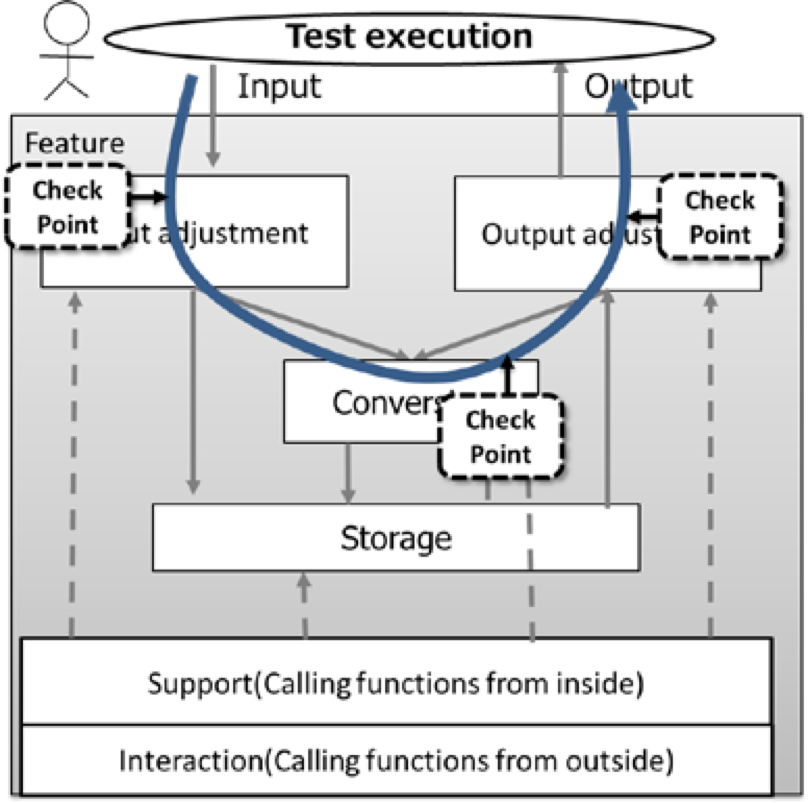
\includegraphics[width=5cm]{./image/D-4-Fig7.png}
 \caption{I/Oテストデータパターンのデータの流れ}
 \label{fig:D-4-Fig7}
 \end{center}
 \end{figure}

しかし,実際に期待結果を確認するチェックポイントは3箇所とは限らない.
なぜなら,入力調整に該当する入力の際に適切な値だけ受け入れることと,変換に該当する計算が適切に行われていることの2つだけであり,出力が適切にされることはチェックポイントとしないといったケースが考えられるためである.

 また,表~\ref{tbl:D-4-tbl1}では,サポートと相互作用についてはデータパターンがプロットされていない.なぜならP1からP9のI/Oデータパターンは単一の入出力の全体像だからである.

論理的機能構造の要素である入力調整,出力調整,変換,貯蔵は,外部観察可能な単一の入出力のみを考慮している分類であるのに対して,サポートと相互作用は,単一の入出力だけではなく,関係する他の処理の呼び出しに着目して仕様項目を特定するための分類である.

サポートと相互作用に分類される仕様項目は,呼び出した後の出力で期待結果を確認する.
呼び出された機能のI/Oテストデータパターンは,論理的に全パターンが発生する可能性がある.
そこで,これまでの研究で行った被験者を使ってテストカテゴリを使った分析手法の習得前と習得後を比較する実験にて使用したテスト分析の講師解答例を同じフォーマットの表に当てはめて,実際の傾向を調査した.

\subsection{これまでの実験データを使った調査}
3章で行った検証実験の結果を基にI/Oテストデータパターンと,テスト条件として特定した論理的機能構造を確認した.
この実験では,ヘッドセットのフィーチャであるボリュームコントロールと,フライト予約システムのフィーチャである新規フライト予約の2種類の異なったAUTを実験に使用した.実験で解答例として作成したテスト分析結果をI/Oテストデータパターンで整理した結果が表~\ref{tab:addlabel-3}である.この結果からわかるとおり,実際に現れたパターンは,P1とP2 とP4とP7だけであり,P1からP9のパターンの全てが現れなかった.またP1でプロットされているのはInput AdjustmentとConversionのみであり,Output Adjustmentに該当する仕様項目は無かった.同様にP2はStorageのみ,P4はConversionとOutput Adjustmentのみであり,各I/Oデータパターンのデータのフローの中で期待結果を確認するチェックポイントが限られていることが確認できた.

% Table generated by Excel2LaTeX from sheet 'Sheet3'
\begin{table}[htbp]
  \centering
  \caption{Add caption}
    \begin{tabular}{|r|p{4em}|l|r|l|r|l|l|}
    \hline
          & \multicolumn{1}{l|}{} & \multicolumn{1}{p{4em}|}{\textbf{入力調整}} & \multicolumn{1}{p{4em}|}{\textbf{出力調整}} & \multicolumn{1}{p{4em}|}{\textbf{変換}} & \multicolumn{1}{p{4em}|}{\textbf{貯蔵}} & \multicolumn{1}{p{2em}|}{\textbf{サポート}} & \multicolumn{1}{p{1.915em}|}{\textbf{相互作用}} \bigstrut\\
    \hline
    \multicolumn{1}{|p{1.5em}|}{\textbf{入力}} & \textbf{外部} & \multicolumn{1}{p{4em}|}{P1(F)} &       & \multicolumn{1}{p{4em}|}{P1(V)} &       &       &  \bigstrut\\
\cline{2-8}          & \textbf{内部} &       &       & \multicolumn{1}{p{4em}|}{P4(V)} &       &       &  \bigstrut\\
\cline{2-8}          & \textbf{外部と内部} & \multicolumn{1}{p{4em}|}{P7(F)} &       & \multicolumn{1}{p{4em}|}{P7(F)} & \multicolumn{1}{p{4em}|}{P7(F)} &       &  \bigstrut\\
    \hline
    \multicolumn{1}{|p{1.5em}|}{\textbf{出力}} & \textbf{外部} &       & \multicolumn{1}{p{4em}|}{P4(F)P7(VF)} &       &       & \multicolumn{1}{p{2em}|}{P1(V)} & \multicolumn{1}{p{1.915em}|}{P1(V)P4(VF)} \bigstrut\\
\cline{2-8}          & \textbf{内部} &       &       &       & \multicolumn{1}{p{4em}|}{P2(VF)} & \multicolumn{1}{p{2em}|}{P2(F)} &  \bigstrut\\
\cline{2-5}\cline{8-8}          & \textbf{外部と内部} &       &       &       &       &       &  \bigstrut\\
    \hline
    \end{tabular}%
  \label{tab:addlabel-3}%
\end{table}%


\subsection{サポートと相互作用に関する考察}
前述したように,論理的機能構造の要素であるサポートと相互作用は,単一の入出力だけではなく,関係する他の処理の呼び出しに着目してテスト条件を特定するための分類である.

TableIIでは,SupportとInteractionに分類できるI/Oテストデータパターンを特定できていなかったが,実際のテスト分析結果から調査した結果,
TableIIIで示したとおり,P1とP2とP4とP7に仕様項目を分類できた.

TableIVには,TableIIIと同実験にてSupportとInteractionに分類した仕様項目を列挙した.

% Table generated by Excel2LaTeX from sheet 'Sheet3'
\begin{table}[htbp]
  \centering
  \caption{Add caption}
    \begin{tabular}{|r|p{8em}|p{4em}|p{4em}|p{5em}|}
    \hline
    \multicolumn{1}{|p{4em}|}{\textbf{フィーチャ}} & \textbf{テスト条件} & \textbf{I/Oテストデータパターン} & \textbf{呼び出し} & \textbf{論理的機能構造} \bigstrut\\
    \hline
    \multicolumn{1}{|p{4em}|}{\textbf{ボリュームコントロール}} & 再生中,通話中以外音量値の調節を無視する & P1    & 割り込み  & サポート \bigstrut\\
\cline{2-5}          & 通話と再生の音量値を調節しても互いに影響を受けない & P1    & リソース共有 & 相互作用 \bigstrut\\
\cline{2-5}          & リセットで音量値がデフォルト値に戻る & P4    & リソース共有 & Interaction \bigstrut\\
    \hline
    \multicolumn{1}{|p{4em}|}{\textbf{新規フライト予約}} & 「既存注文検索」へ注文が反映すること & P4    & 他への反映 & Interaction \bigstrut\\
\cline{2-5}          & 「注文件数グラフ」へ注文が反映すること & P4    & 他への反映 & Interaction \bigstrut\\
\cline{2-5}          & 「注文履歴」へ注文が反映すること & P4    & 他への反映 & Interaction \bigstrut\\
\cline{2-5}          & 登録時にチケット在庫なしの場合エラーになること & P1    & 他処理連動 & Support \bigstrut\\
\cline{2-5}          & 注文挿入中に強制終了すると処理をロールバックすること & P2    & 他処理連動 & Support \bigstrut\\
    \hline
    \end{tabular}%
  \label{tab:addlabel}%
\end{table}%

サポートと相互作用として特定する仕様項目の傾向について以下のような考察が出来る.

サポートは,フィーチャセットでのテスト実行時のアクションによって内部的に呼び出される別の処理の結果確認のことを指している.
この例では,全てテスト対象の入力に対して結果を返すだけであるため,I/OテストデータパターンはP1としている.

一方,相互作用は,テスト実行時のアクションによる副作用を,他フィーチャに対するアクションにて呼び出して確認することを指している.

この例では,ボリュームコントロールの2つの仕様項目は,副作用を確認する際に,該当する他フィーチャにてテスト実行時に外部から入力を与えて結果を確認するためP1にしている.フライト予約システムの場合は,新規フライト予約にて登録した新規予約が反映していることを他のフィーチャにて確認することを指しているが,テスト実行の際は該当のフィーチャに対して外部入力を与えずともすでに保存された結果の出力で確認ができるためP4としている.

サポートに該当する仕様項目の特定に使う呼び出しのきっかけと相互作用に該当する仕様項目の特定に使う呼び出しのきっかけを整理して,I/Oテストデータパターンとの対応がわかるようにした.
整理した結果をTableVに示す.
% Table generated by Excel2LaTeX from sheet 'Sheet3'
\begin{table}[htbp]
  \centering
  \caption{Add caption}
    \begin{tabular}{|p{4em}|c|p{4em}|p{4em}|c|}
    \hline
    呼び出し  & \multicolumn{1}{p{4em}|}{割り込み} & リソース共有 & 他への反映 & \multicolumn{1}{p{4em}|}{他処理連動} \bigstrut[t]\\
    \multicolumn{1}{|l|}{} &       & \multicolumn{1}{r|}{} & \multicolumn{1}{r|}{} &  \\
    論理的機能構造 &       & \multicolumn{1}{r|}{} & \multicolumn{1}{r|}{} &  \bigstrut[b]\\
    \hline
    サポート  & \multicolumn{1}{p{4em}|}{○} & \multicolumn{1}{c|}{} & \multicolumn{1}{c|}{} & \multicolumn{1}{p{4em}|}{○} \bigstrut\\
    \hline
    相互作用  &       & ○     & ○     &  \bigstrut\\
    \hline
    \end{tabular}%
  \label{tab:addlabel}%
\end{table}%

TableVには,各仕様項目を特定する際のきっかけとなる呼び出し方法を列挙した.
サポートに該当する仕様項目の特定に使う呼び出しのきっかけと相互作用に該当する仕様項目の特定に使う呼び出しのきっかけを整理することで,他のAUTに適用する際に活用できると考えられるためである.
呼び出しのきっかけとI/Oテストデータパターンの組み合わせはTableVのように整理できた.

\newpage
\section{I/Oテストデータパターンを使ったテスト分析の実験} \label{sec:4-2}
% 本章の実験では,現実のプロジェクトで作られたテストケースと,今回提案するI/Oテストデータパターンを使ったテスト分析結果を比較し,手法の効果を分析した.
\subsection{実験の目的} \label{sec:4-2-1}

これまでの実験では,被験者の学習過程に対する効果を検証してきた.
また,実験用に用意した小さなサンプルを利用してきた.

この実験は,今回提案しているテストカテゴリにI/Oテストデータパターンを使う手法が現実のテスト設計と比較して網羅的にテスト条件を特定できることを目的とする.
そのために現実のテスト設計の結果と,I/Oテストデータパターンを使った分析結果を比較する.

この実験は以下の目的で行う.

\subsubsection{I/Oテストデータパターンの効果実証}
\begin{itemize}
\item 目的:今回提案しているテストカテゴリにI/Oテストデータパターンを使う手法が,現実のテスト設計と比較して網羅的に仕様項目を特定できることを確認する.
\item 評価方法:現実のテスト設計の結果と,I/Oテストデータパターンを使った分析結果を比較する.
\end{itemize}

\subsection{実験の題材} \label{sec:4-2-3}

実験対象のテスト対象は,実在するオンラインのモバイル写真共有アプリケーションを使った.
簡単なサンプルでは出現しないデータパターンもあるため,現実の複雑なアプリケーションを対象にした.
全機能のうち,「アップロード(デバイス上の写真をオンラインサーバへアップロード)」,「グリッドビュー(オンライン上の写真をデバイスにてサムネイルの一覧として閲覧)」という二つのFeatureをテスト対象として選択した.
この二つの機能を選択した理由は,データの内部への投入を行う機能とデータの照会のみ行う機能とで,I/Oテストデータパターンの出現傾向が異なること調査することが出来ると考えたためである.
このモバイル写真共有アプリケーションの開発にて実際に使われたテストケースと,提案する手法で分析した結果を比較する.

\subsection{実験の実施手順}
実験は以下の手順で行なった.

\begin{itemize}
\item 実際に作られたテストケースをテスト条件にまとめなおす.
\item フィーチャセットで使われる入力データ,出力データを明らかにする.
\item I/Oテストデータパターンを付与する.
\item 論理的機能構造とI/Oテストデータパターンを使ってテストベースを分析する.
\end{itemize}

以降,各手順で行う内容を具体的に述べていく.

\subsection{1) テストケースのテスト条件への変換}

今回の実験で使う成果物には,テストケースのみであり,テスト分析のアウトプットとなるテスト条件の一覧はなかった.
テストケースは,入力値や事前条件を組み合わせた複数のインスタンスであるため,今回の実験のためにテスト分析でのアウトプットである仕様項目と期待結果としてまとめなおす必要がある.
そのため,比較元のテストケースは,今回の実験のためにテスト分析でのアウトプットであるテスト条件になるようまとめなおした.
まとめ直す際には,図~\ref{fig:D-4-Fig8}のように,テストケースの要素を整理し,同じアクションを行い,同じ期待結果を確認しているテストケースはひとつの仕様項目としてまとめた.

\begin{figure}[htbp]
\begin{center}

\includegraphics[width=12cm]{./image/D-4-Fig8.png}
\caption{テストケースから仕様項目をまとめる方法の説明}
\label{fig:D-4-Fig8}
\end{center}
\end{figure}

現場で作られたテストケースの数は,アップロードが491ケース,グリッドビューが151ケースであった.仕様項目として整理した結果,アップロードが59項目,グリッドビューが22項目の仕様項目となった.
このように数量が変わる理由は,たとえば「デバイスからサーバーへ画像ファイルをアップロードして保存が出来ること」というひとつの仕様項目に対して,テストケースは,画像の種類(Jpg,Bmpなど),画像のサイズ,アップロードする画像の枚数,画像情報のパターン(ファイル名,撮影日など)といったテストパラメータを組み合わせたものがテストケースとなっているためである.

\subsection{2)入力データ,出力データの特定}
フィーチャセットであるアップロードとグリッドビューのテストベースを分析し以下の4つを入力データ,出力データとして扱うこととした.
\begin{itemize}
 \item 画像データ
 \item 画像の情報
 \item 設定データ
 \item 外部コマンド
\end{itemize}

\subsection{3)I/Oテストデータパターン付与}
特定した入力データと出力データは,2)で明らかにした仕様項目に対してFig.9.のリストのようにInput data ,Output dataというカラムに追記していった.テスト実行時の追記したデータの流れをシミュレーションし,該当するI/Oテストデータパターンを明らかにした.図〜ref {fig:D-4-Fig9}は,ソート順の情報を外部から入力し,内部からの入力となる画像データと一緒になり,外部にソートした画像データを表示している例である.この場合のI/OテストデータパターンはP7となる.

\begin{figure}[htbp]
\begin{center}
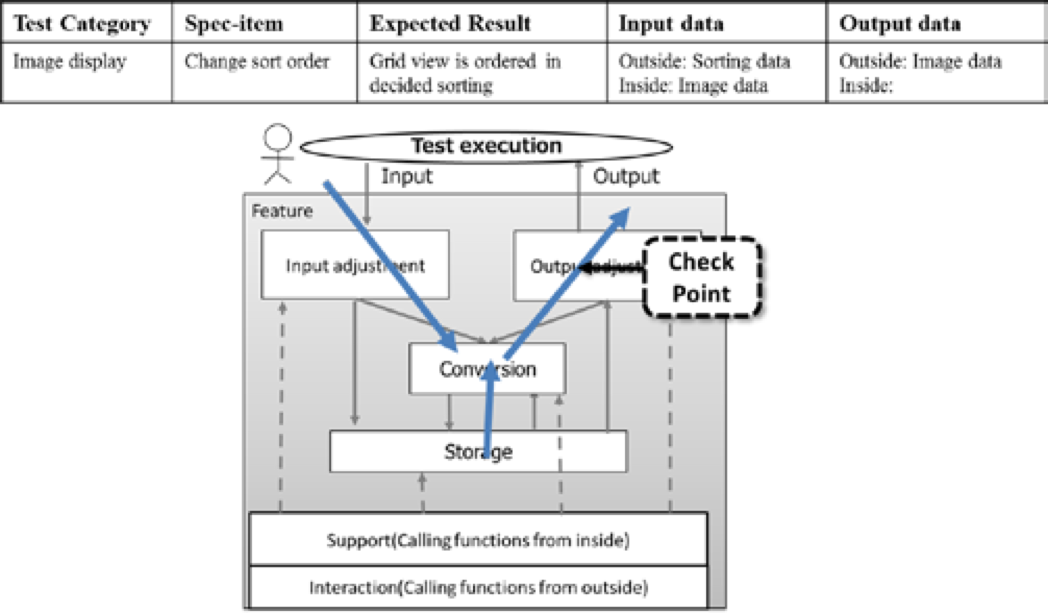
\includegraphics[width=10cm]{./image/D-4-Fig9.png}
\caption{仕様項目に入力データと出力データを加える方法の説明}
\label{fig:D-4-Fig9}
\end{center}
\end{figure}

\subsection{I/Oテストデータパターンを使ったテストベース分析}
I/Oテストデータパターンと既存の分析手法であるテストカテゴリを併用してテスト分析を行う.
作業ステップは以下のとおりである:
\begin{itemize}
 \item TableVI,VIIのようにテストカテゴリを特定する
 \item テストカテゴリ毎に入力データと出力データを明らかにする
 \item I/Oテストデータパターンごとのデータの流れをシミュレーションして仕様項目を選択する
 \item 現場のテストケースを分析した結果をテストカテゴリに分類し,差異を比較する.
\end{itemize}
サポートと相互作用については,テストカテゴリとして特定したTriggerで呼び出す機能から仕様項目を選択した.

\subsection{1)IOテストデータパターンの効果実証の結果}
テストカテゴリとI/Oテストデータパターンを使ったテストベースの分析を行った結果をにまとめた.

% Table generated by Excel2LaTeX from sheet 'Sheet3'
\begin{table}[htbp]
  \centering
  \caption{Add caption}
    \begin{tabular}{|p{4em}|p{4em}|p{4em}|p{4em}|p{4em}|p{2em}|p{1.915em}|p{4em}|p{4em}|p{4em}|}
    \hline
    \multicolumn{1}{|r|}{} & \multicolumn{1}{l|}{P1} & \multicolumn{1}{l|}{P2} & \multicolumn{1}{l|}{P3} & \multicolumn{1}{l|}{P4} & \multicolumn{1}{l|}{P5} & \multicolumn{1}{l|}{P6} & \multicolumn{1}{l|}{P7} & \multicolumn{1}{l|}{P8} & \multicolumn{1}{l|}{P9} \bigstrut\\
    \hline
    アップロード & ○     & ○     & ○     & ○     & X     & ○     & ○     & X     & ○ \bigstrut\\
    \hline
    グリッドビュー & ○     & X     & X     & ○     & X     & X     & ○     & X     & ○ \bigstrut\\
    \hline
    \end{tabular}%
  \label{tab:addlabel}%
\end{table}%


今回のフィーチャセットであるアップロードとグリッドビューの 両方でテストカテゴリとI/Oテストデータパターンを使ったテストベースの分析が適用できた.そして,両方のフィーチャにて,現実のテスト対象に おけるテスト設計と比較し,現場のテスト設計に仕様項目が不足していることが実証できた.分類に利用したI/Oテストデータパターンは,P5とP8を除く全てであった.


実プロジェクトのテスト条件との比較をした結果を図~\ref{fig:D-4-Fig10}に示す.
両者を比較すると,I/Oテストデータパターンを利用したテスト分析の結果が実プロジェクトより多くのテスト条件を選択できたことが確認できている.

\begin{figure}[htbp]
\begin{center}
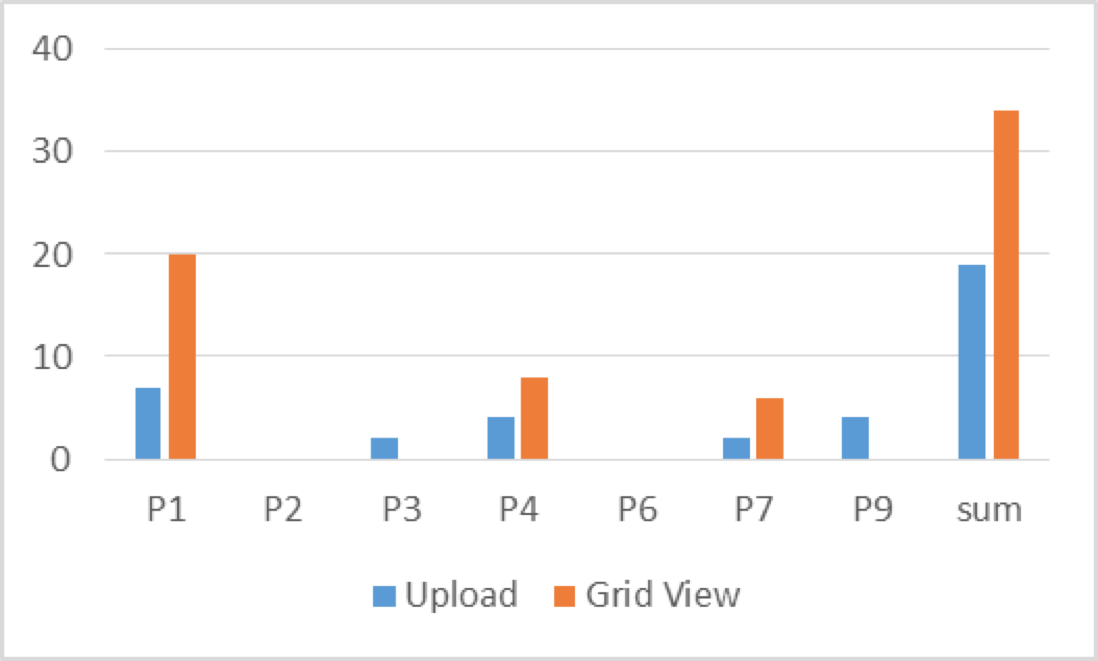
\includegraphics[width=10cm]{./image/D-4-Fig11.png}
\caption{IOテストデータパターンごとの違い}
\label{fig:D-4-Fig10}
\end{center}
\end{figure}

\subsection{I/Oテストデータパターン毎の出現傾向の評価}
現実のプロジェクトで作られたテストケースとテストカテゴリとI/Oテストデータパターンを使ったテストベースの分析結果をP1からP9の分類で出現割合を比較した結果が,Table IX.である.

現実のプロジェクトにて不足していたテスト条件には,I/Oテストデータパターン別にみるとP1が特にテストカテゴリと実プロジェクトの差異が大きいことがわかる.P1 は外部からの入力を行い,外部に出力する最も単純なパターンであり,I/O テストデータパターンから見ても単純なことを確認するテスト条件が漏れている.
\begin{figure}[htbp]
\begin{center}
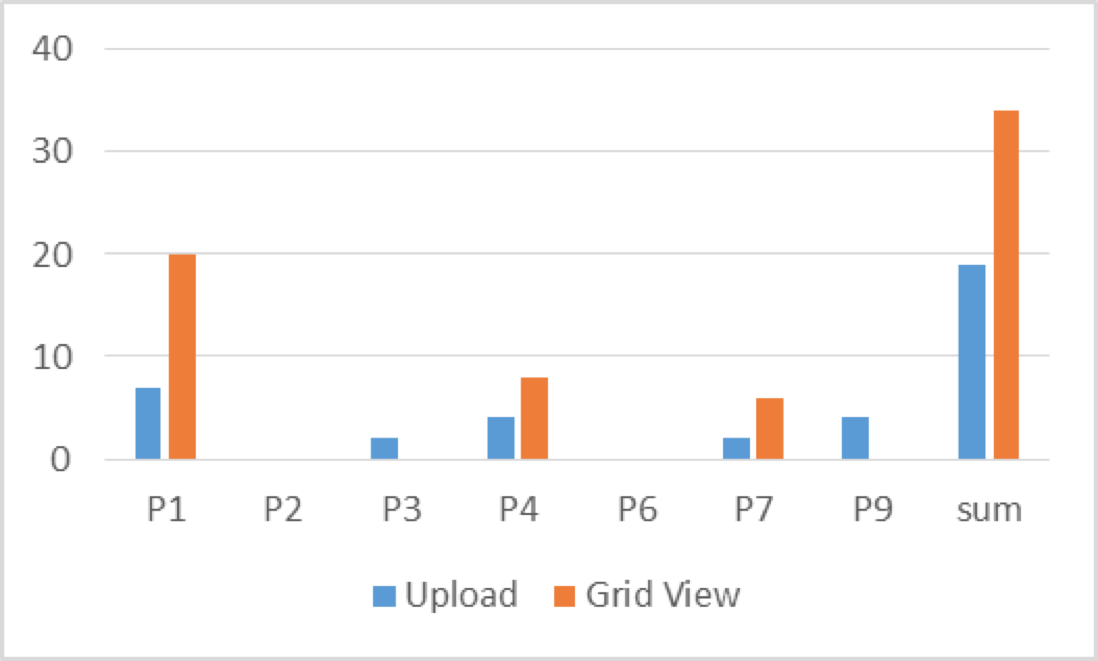
\includegraphics[width=10cm]{./image/D-4-Fig11.png}
\caption{IOテストデータパターンごとの違い}
\label{fig:D-4-Fig11}
\end{center}
\end{figure}

\subsection{現実のプロジェクトにて不足していた仕様項目}
TableXには,現実のプロジェクトにて不足していた仕様項目をいくつか抜粋して列挙した.これらの仕様項目は,全て今回のデータのI/Oのシミュレーションを行い網羅的にテストベースを確認することで特定できたものである.不足していた仕様項目には,論理的機能構造の要素別に見てもInput Adjustment, Output Adjustmentといったメッセージが現れることや入力制御といった単純なことを確認する仕様項目でも漏れているものもあることが確認できる.

一般的に,仕様項目のリストを作成せずにテストケースを作った場合,テストケースのままでは数量の多さから網羅すべき仕様項目の見易さが低下するため,仕様項目の数が不足することが多い.
実験結果も同様の傾向となった.

\newpage
\section{終わりに}
 本論文では,テスト実行時のデータI/Oの要素で分類し網羅的に分析する方法を提案した.そして,現場のテストプロジェクトのテストケースを使い,提案した方法の実証を試みた.結果的に,提案した方法で特定した仕様項目と実プロジェクトで作られるテストケースと比較して,不足している仕様項目の発見が可能であることが確認できた.I/Oテストデータパターンを活用したテスト分析をするためには,まだ多くのサンプルを入手し,全てのI/Oテストデータパターンをナレッジにする必要がある.ナレッジにすることで,テスト分析にて仕様項目を効率よく特定するルールを確立させていきたい.
